\subsection{How to Graph with Transformations}
\begin{example}[Examples]
  \hfill
  \begin{enumerate}
  \item $f(x) = -\frac{1}{2}|x - 3|+ 2$ \\
    $\text{Key Points} = (1, 1) \, (0, 0) \, (-1, 1)$ \\
    \textbf{Steps: }
    \begin{enumerate}
    \item Up 2.
    \item Right 3.
    \item Vertical Compression.
    \item Reflect About $x$.
    \end{enumerate}
    \hfill
    \begin{center}
      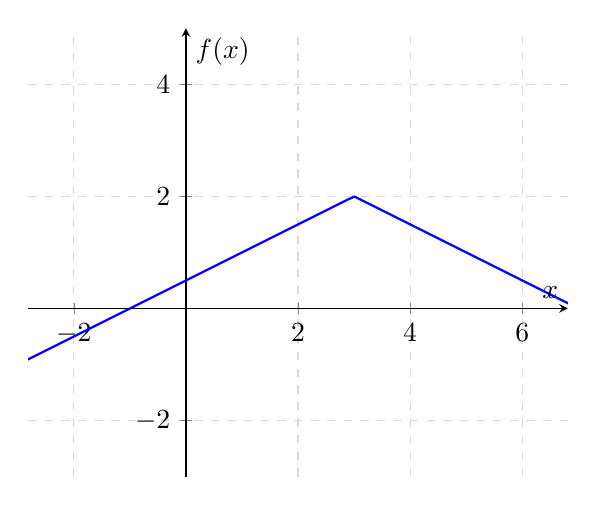
\begin{tikzpicture}
	\begin{axis}[
	    axis lines = center,
	    xlabel = $x$,
	    ylabel = $f(x)$,
	    xmin = -2, xmax = 6,
	    ymin = -3, ymax = 5,
	    grid = both,
	    grid style = {dashed, gray!30},
	    axis equal
	  ]
	  \addplot [domain=-5:8, samples=100, thick, blue] {-0.5*abs(x-3)+2};
	\end{axis}
      \end{tikzpicture}
    \end{center}
  \item $g(x) = -\frac{1}{3}(x + 1)^3 - 1$ \\
    $\text{Key Points} = (1, 1) \, (0, 0) \, (-1, -1)$ \\
    \textbf{Steps: }
    \begin{enumerate}
    \item Down 1.
    \item Left 1.
    \item Vertical Compression.
    \item Reflect about $x$.
    \end{enumerate}
    \hfill
    \begin{center}
      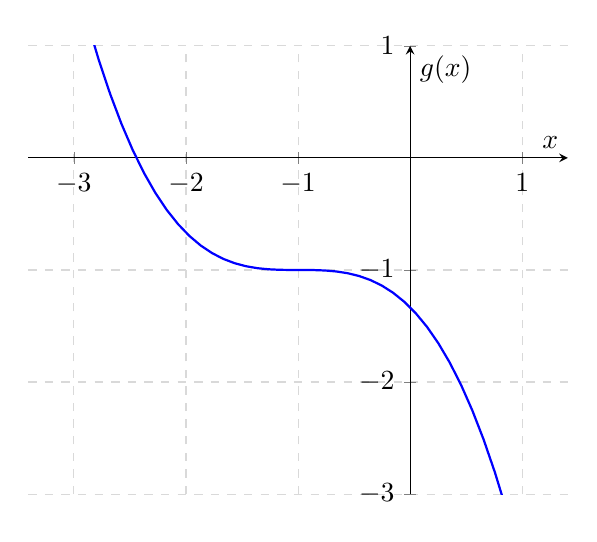
\begin{tikzpicture}
	\begin{axis}[
	    axis lines = center,
	    xlabel = $x$,
	    ylabel = $g(x)$,
	    xmin = -3, xmax = 1,
	    ymin = -3, ymax = 1,
	    grid = both,
	    grid style = {dashed, gray!30},
	    axis equal
	  ]
	  \addplot [domain=-5:5, samples=100, thick, blue] {(-1/3)*(x+1)^3-1};
	\end{axis}
      \end{tikzpicture}
    \end{center}
  \item $f(x) = \frac{3}{x - 2} + 1$ \\
    $f(x) = \frac{3}{x  - 2} + 1 \to 3 . \frac{1}{x - 2} + 1$ \\
    $\text{Key Points} = (1, 1) \, (-1, -1) $ \\
    \textbf{Steps: }
    \begin{enumerate}
    \item Up 1.
    \item Right 2.
    \item Vertical Stretch.
    \end{enumerate}
    \hfill
    \begin{center}
      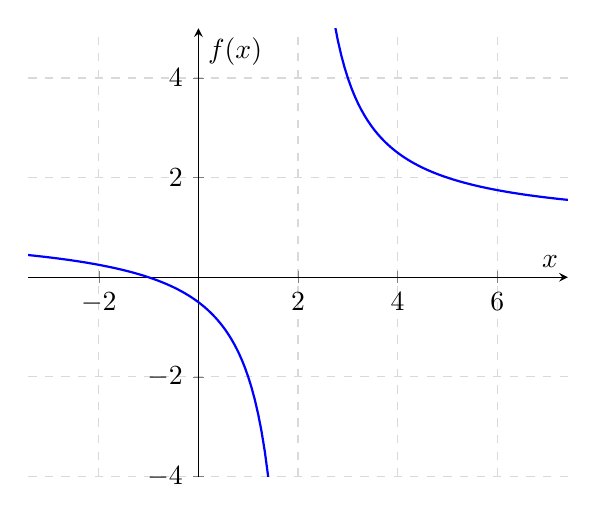
\begin{tikzpicture}
	\begin{axis}[
	    axis lines = center,
	    xlabel = $x$,
	    ylabel = $f(x)$,
	    xmin = -2, xmax = 6,
	    ymin = -4, ymax = 5,
	    grid = both,
	    grid style = {dashed, gray!30},
	    axis equal
	  ]
	  \addplot [domain=-5:1.6, samples=100, thick, blue] {3/(x-2)+1};
	  \addplot [domain=2.4:9, samples=100, thick, blue] {3/(x-2)+1};
	\end{axis}
      \end{tikzpicture}
    \end{center}
  \item $g(x) = 2 \sqrt{1 - x} + 3$
    $g(x) = 2 \sqrt{1 - x} + 3 \to 2 \sqrt{-x + 1} + 3$\\
    $g(x) = 2 \sqrt{-(x-1)} + 3$ \\
    $\text{Key Points} = (1, 1) \, (0, 0)$ \\
    \textbf{Steps: }
    \begin{enumerate}
    \item Up 3.
    \item Right 1.
    \item Reflect About $x$.
    \item Vertical Stretch.
    \end{enumerate}
    \hfill
    \begin{center}
      \begin{tikzpicture}
	\begin{axis}[
	    axis lines = center,
	    xlabel = $x$,
	    ylabel = $g(x)$,
	    xmin = -3, xmax = 5,
	    ymin = -1, ymax = 7,
	    grid = both,
	    grid style = {dashed, gray!30},
	    axis equal
	  ]
	  \addplot [domain=-4:1, samples=100, thick, blue] {2*sqrt(1-x)+3};
	\end{axis}
      \end{tikzpicture}
    \end{center}
  \end{enumerate}
\end{example}
